\section{Introduction}
A major goal of the Habitable Worlds Observatory is to characterize the orbits
and atmospheres of as many habitable worlds as possible. To do this it will use
the direct imaging exoplanet detection technique since it provides the best
opportunity for full spectral characterizations. However, exoplanets are among
the faintest objects that have been the primary targets of an observation and
will require days to weeks of integration time. To complicate matters further,
multiple observations will be required to pin down the orbit of an exoplanet
before deciding on the best time to do a full spectral characterization.
Allocating the time required for spectral characterizations is therefore
incredibly costly given the considerable cost of construction, operation, and
alternative science objectives for a mission like the Habitable Worlds
Observatory.

Early in the life of a mission, many design decisions are driven by modeling
how the different aspects of a mission impact the science goals of a mission.
For exoplanets this can be seen in papers discussing the tradeoffs between the
diameter of the primary mirror and the number of exoplanets  that will be
detected, often called the "mission yield". Yield modeling studies will be
important to the success of the Habitable Worlds Observatory and two primary
tools have been created to study the mission yield of space-based direct
imaging missions, \code{EXOSIMS} and AYO. Both tools were built around calculating the
mission yield with no prior information about the planetary system of the
available target stars. However, it is likely that by the time of launch there
will be a considerable amount of information for some planetary systems.

Considerable effort is being invested into improving the radial velocity (RV)
exoplanet detection method to discover more exoplanets, and it has been
identified as the most promising method to detect Earth-like exoplanets. The
mission concept studies of both HabEx and LUVOIR identified the collection of
precursor RV data as integral to increasing the number of exoplanets detected.


The most recent study, \citet{morganExplorationExpectedNumber2022a}, showed
that having precise orbital information from RV before launch can improve yield
considerably [expand with study specifics]. This study is best thought of as an
upper bound for the mission yield improvement due to RV data because it assumed
full orbital recovery. Assuming full orbital recovery comes with many benefits
for computational time and is done probabalistically based on research on what
planets are likely to be discovered depending on the amount and quality of RV
data collected. This makes it a quick and robust way to determine which planets
are likely to be detected. 

The drawback of using full orbital recovery for yield modeling is that fitting
orbits to RV data only estimates certain orbital parameters. The standard set
is period $T$, time of conjunction $T_c$, argument of periapsis $\omega$,
eccentricity $e$, and minimum mass $M_p \sin{i}$. The minimum mass quantity
combines two parameters that impact direct imaging and estimations of an
exoplanet's brightness and location cannot be exact without separating the
planet mass and inclination. Without non-RV data those quantities cannot be
separated. An additional complication is that orbit fits have uncertainties on
fitted parameters which should be accounted for when scheduling observations.

A way of accounting for the inclination and mass ambiguity and uncertainty was
shown in \Cref{cha:first_paper}. The uncertainties from the fitting
process and an inclination prior are used to create a set of orbits that the
planet that created the radial velocity curve is most likely to be on. Then the
probability of detection is calculated, similar to the completeness metric
established in \citet{Brown2005d}, by propagating the orbits in that set and
comparing each orbit's brightness and planet-star separation to a direct
imaging telescope's sensitivity limits.

Fully simulating direct imaging missions with precursor RV requires simulating
the many RV observing runs that collect RV data for the stars in the direct
imaging target list. Real RV data cannot be used because the full planetary
systems that generate real RV data are unknown.

\section{Methods}
To incorporate precursor data realistically we must create synthetic planetary
systems around the stars in the simulation, simulate the collection of RV data,
do blind RV fitting of the RV data to create fits for scheduling, calculate the
probability of detection for each fit during the direct imaging mission, and
finally use the probability of detection information to create a direct imaging
observation schedule, and finally simulate the mission using a direct imaging
mission simulator. The major code pieces are \code{EXOSIMS} for planet generation and
direct imaging observation simulations, \code{RVSearch} for blind fitting RV data, and
the new package \code{RVtoImaging} that handles RV observations and scheduling. An
overview of the software package is shown in \Cref{fig:rv2imgflowchart}.

\begin{figure}
  \begin{center}
    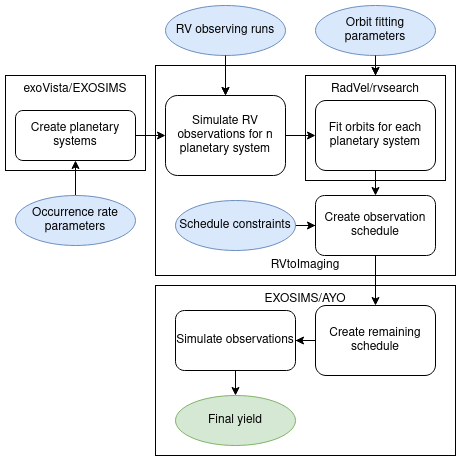
\includegraphics[width=0.95\textwidth]{ch4/figures/flowchartwhite.png}
  \end{center}
  \caption{Framework for simulating the use of precursor radial velocity data
  for direct missions.}
  \label{fig:rv2imgflowchart}
\end{figure}

The code is built to save anything that may be used again to reduce computation
time. It has detailed logging information printed for all steps of the process
and it manages a complex file structure to ensure that data can be quickly
found. Inputs are managed as a set of dictionaries from a driver script that is meant
to be easily modified.

\subsection{Planetary system generation}

The synthetic systems used in this study are created with \code{EXOSIMS}'s
implementation of the nominal occurrence rates from Dulz \citep{dulzJointRadialVelocity2020}. Full systems
are generated and then imported into a python package, exoverses, which was
created to work as an intermediary between planetary system generators and
\code{RVtoImaging}. Currently exoverses supports exoVista and \code{EXOSIMS}.

\subsection{RV Dataset}

The RV dataset is composed of user-defined RV observing runs and a set of
target stars. These observing runs are defined by
\begin{itemize}
  \item Bad weather probability
  \item Exposure time
  \item Min and max airmass
  \item Minimum observations per star
  \item Observatory location
  \item Start and end time
  \item RV precision terms
  % \item Observation scheme
\end{itemize}
This section of code makes uses the \code{astroplan} python package to
determine observability of the target stars for the observatory location and
airmass constraints \citep{morrisAstroplanOpen2018}. The simple observation
scheme takes in an average number of observations per star per year and assigns
those observations to discrete blocks that are equal in length to the exposure
time. Observations cannot overlap and stars are only observed once per night.
The constraint observation scheme is set up to simulate having a set number of
observing nights. Users define a set number of nights for observation and the
nights are drawn randomly within the given time frame. Then we set up an
optimization problem that maximizes the number of observations on each given
night and the number of stars that are observed a user-defined minimum number
of times, subject to the constraints that no star should be observed more than
once per night and no observations can overlap. The optimization problem is
solved using the Constraint Programming Satisfiability (CP-SAT) solver from
OR-Tools \citep{perronORTools2022}. After all observations are assigned, each
night gets a random draw of bad weather, if there is bad weather then the
observations from that night do not occur.

After a schedule is created we simulate the observation of the stars. For each
target we calculate the true anomaly, $\nu$, of all planets in the system and
calculate the star's radial velocity as 
\begin{equation}
v_s = \Sigma_i \left(K_i \left(e_i
\cos(\omega_i) + \cos(\nu_i + \omega_i)\right)\right) \,
  \label{eq:system_rv}
\end{equation}
where $K_i$, $e_i$,
$\omega_i$ are the RV semi-amplitude, eccentricity, and argument of periapsis
respectively of planet $i$. Each observing run is defined with a number of
error terms that are added in quadrature to get a final RV precision. Then we
treat the noise sources as uncorrelated and draw RV errors for each measurement
with the final RV precision as the one $\sigma$ value for a Gaussian
distribution centered on zero. There are time-correlated noise signals in real
RV data which can be corrected. However, this is done in a case-by-case basis
and is difficult to scale \citep{guptaTargetPrioritization2021}. Additionally,
we would be adding time-correlated noise with a Gaussian processes and then
removing them with the same Gaussian process analysis
\citep{aigrainGaussianProcess2022}. It is possible to deliberately chose
different kernel functions for the Gaussian process used in generation and the
Gaussian process used in fitting to add noise, but it is much more straight
forward to treat the time-correlated noise terms as a single value of RV
uncertainty to be defined by the user.

This process of generating RV data is repeated for each target star in the
observing run. Then the full process is repeated for every observing run in the
RV dataset. \code{RVtoImaging} is set up so that RV observing runs are deterministic
for a given generated universe and observing run parameters, allowing a user to
easily test how different combinations of observing runs impact fitting and
ultimately direct imaging scheduling. It is easy to compare how an individual
observing run impacts the final fit of a planetary system by adding or removing
it from the script driving the simulation.

\subsection{Blind RV fitting}

\code{RVtoImaging} does a blind search for every star with observations in the RV
dataset. A number of tools exist to do RV fitting, but systematic
blind searching without any prior information limits the number of tools. The
one best suited for this work is \code{RVSearch} which was created for the California
Legacy Survey \citep{rosenthalCaliforniaLegacy2021}. \code{RVSearch} is built on top of the radvel library, a python
package that uses the Markov Chain Monte Carlo (MCMC) simulations to fit
Keplerian orbits to RV data with confidence intervals. \code{RVSearch} sets up the
log-likelihood function as \citep{rosenthalCaliforniaLegacy2021} 
\begin{equation}
\ln(\mathcal{L}) = -\frac{1}{2}
\Sigma_i \left[ \frac{\left(v_i - m(t_i) - \gamma_D\right)^2}{\sigma_i^2} +
\ln\left(2 \pi \sigma_i^2\right)\right]
  \label{eq:likelihoodfun}
\end{equation}
where $i$ is the observation index,
$v$ is the RV measurement, $m$ is the model RV, $\gamma_D$ is the instrument's
offset, and $\sigma$ is the root-mean-square of error terms. The model is
defined as 
\begin{equation}
m(t) = \Sigma_n K(t|K_n,P_n,e_n,\omega_n,T_{c,n}) +
\dot{\gamma}(t-t_0) + \ddot{\gamma}(t-t_0)^2
  \label{eq:rv_model}
\end{equation}
where $n$ is the fitted orbit
index, $K(t|K_n,P_n,e_n,\omega_n,T_{c,n})$ is the RV signal for planet $n$, $P$
is the period, $T_{c,n}$ is the time of conjunction, $\dot{\gamma}$ is a linear
trend term, $t$ is the time of interest, $t_0$ is a reference time, and
$\ddot{\gamma}$ is a quadratic trend term. \code{RVSearch} works by creating a
Bayesian information criteria (BIC) periodogram of the RV data to identifying
the strongest periodic signals. \code{RVSearch} calculates the BIC as 
\begin{equation}
BIC = k
\ln\left(n_{obs})\right) - 2\ln{\mathcal{L}}
  \label{eq:bic}
\end{equation}
where $k$ is the number of free
parameters and $n_{obs}$ is the number of observations. With the strongest
periodic signal identified it does a maximum *a posterior* fit to determine the
most likely Keplerian parameters for the planet that generated the periodic
signal. Planets are added to a collective posterior until there are no periodic
signals left that improve the BIC, or until it reaches the maximum number of
planets it is allowed to search for.

After all significant periodic signals in the RV data have been identified,
\code{RVSearch} refines them and determines confidence intervals by performing a MCMC
simulation with all planet parameters free. This MCMC process is done using the
emcee library \citep{emcee} which is a popular python implementation of the affine
invariant ensemble sampler \citep{Goodman2010}. This process is very computationally costly,
because the search space increases considerably with every new planet and the
periodogram does a maximum *a posterior* fit at every test period with all
parameters of previously added planets free.

\code{RVtoImaging} works on forked versions of \code{RVSearch} and \code{RadVel} that were created
for performance reasons. The \code{RVSearch} fork was created primarily because the
current \code{RVSearch} package is pegged to \code{RadVel} version 1.3.8 and does not work
with \code{RadVel} versions 1.4.x which improved performance by vectorizing a number
of calculations. Further, the fork modifies some class attributes so that
\code{RVtoImaging} can tell things such as whether the MCMC chains converged. The
\code{RadVel} fork has a number of minor optimizations and a major optimization in the
form of a C version of the log likelihood function that implements the fast
eccentric anomaly solver from orvara \citep{brandtOrvaraEfficient2021} which is
based on \citet{raposo-pulidoEfficientCode2017}. An experimental feature was
added to the RVS

There are two major bottlenecks in this process. The first is that MCMC does
not scale well with multiple cores because emcee exits parallelization every
time it checks for convergence. Because of this it is better to spawn multiple
processes that have between 5-10 cores because any benefit gained by
parallelizing the periodogram search is offset by the wasted time in MCMC. The
more limiting bottleneck is that MCMC convergence drops considerably as more
planets are added. An unconverged MCMC run will give biased confidence
intervals which are of primary importance for estimating when a planet is
detectable so we will not consider unconverged chains valid in this work.
Convergence is rare, less than 20\%, when the number of planets in the search
space is five or more. When running multi-planet fits we found it best to cap
the number of planets in the search to four, which results in a 57\%
convergence rate and a standard run time of 30-40 minutes per search.

A major drawback of those computational limitations is that as more planets are
identified the parameter distributions of all planets become better
constrained. Additionally, by capping the number of planets fitted per system
to four we limit the number of planets we will consider in the scheduling step,
lowering the maximum yield. This is an unfortunate limitation because it restricts
our ability to fully understand the impact of different RV precision value.
This limitation is a necessary consequence of fitting tools prioritizing
precision over efficiency.

\subsection{Probability of Detection}

Probability of detection is calculated in the manner laid out in
\Cref{cha:accurate_pdet} paper), which is an adaptation of the "completeness"
metric described in \citep{brownSingleVisitPhotometric2005} . Using the MCMC
chains from the fitting process we generate a representative sample of orbits
that are consistent with the observed RV data for each planet fitted. If the
fit is an accurate description of the consistent orbits, we can propagate the
consistent orbits in time and when they are all detectable the true planet will
be detectable as well. \code{RVtoImaging} is set up to work the "Credible Interval" or
the "Multivariate Gaussian" methods of constructing consistent orbits.
Calculating probability of detection relies on a specific set of direct imaging
observatory parameters, since an orbit is considered detectable if it meets the
criteria laid out in \Cref{cha:accurate_pdet} The $\Delta\textrm{mag}_0(\alpha,
t_{\textrm{int}}, n_\textrm{Z}, n_\textrm{EZ})$ values are found for a specific
telescope using \code{EXOSIMS}'s \code{calc\_dMag\_per\_intTime} function. 

We do not attempt to create interpolants for all four inputs to
$\Delta\textrm{mag}_0$, instead calculating a 2d interpolant that takes in
$\alpha$ and $t_\textrm{int}$ values and returns the $\Delta\textrm{mag}_0$. An
interpolant is calculated for a discrete set of $n_\textrm{Z}$ values and a
single $n_\textrm{EZ}$ values. Extra zodiacal light brightness is a function of
the separation $\alpha$ and drops off with a $1/r^2$ term as discussed in
\citet{starkMaximizingExoEarthCandidate2014} so at every separation $\alpha$ we
calculate the corresponding extra zodiacal light surface brightness. Then when
calculating the $\Delta\textrm{mag}_0$ values at an observation time $t$ we
pick the interpolant that is closest to the current zodiacal light surface
brightness for the star at $t$, because it is a function of the telescope's
position in orbit, and the number of zodis assumed to be in the planetary
system. Ideally, we would be assigning the number of zodis in the system
probabilistically for each constructed orbit, but this is outside the scope of
this work as it adds a tremendous amount of complexity to the code. Instead we
treat the number of zodis in the planetary system as an input and assume it to
be constant when calculating the $P_\textrm{det}$ values for all planetary
systems.

In \code{RVtoImaging} the user defines an \code{EXOSIMS} input script for telescope
parameters, the consistent orbit construction method, a minimum integration
time, a maximum integration time, a start time, and an end time. Then the
orbits are repeatedly propagated between the start and end times and
$P_{\textrm{det}}(t, t_{\textrm{int}}, n_\textrm{Z}, n_\textrm{EZ})$ is
calculated for integration times spaced between the minimum and maximum. The
$P_{\textrm{det}}$ information for all planets around a star are stored as a
three dimensional array that is indexed on the planet number (assigned during
RV fitting), $t$, and $t_{\textrm{int}}$.

\subsection{Scheduling Observations}

Our aim in this work is to schedule observations of the fitted planets in a way
that is consistent with the observation strategies outlined in the HabEx and
LUVOIR studies \cite{gaudiHabitableExoplanetObservatory2020,TheLUVOIRTeam2019}.
They outlined a multi-tiered process that begin by using the telescope's
detection observing mode, as opposed to the observing mode for atmospheric
characterization, to better resolve the orbits of planets in the initial
portion of the mission. Work has shown that it takes 3-4 direct imaging
observations to determine an exoplanet's orbit to 10\%
\citep{bluntOrbitsImpatient2017}, and fewer are required when precursor data
exists \citep{gaudiHabitableExoplanetObservatory2020}. Further, it's important
to try and space out observations of a planet, as gathering 3 observations of
an Earth-like planet on 3 consecutive days will result in a considerably worse
fit than 3 observations made months apart.

\subsubsection{Decision variables}

We use this information to drive our scheduling task, attempting to get decent
orbital coverage of as many fitted planets as possible. This scheduling is done
with constraint programming, using the CP-SAT solver from
OR-Tools\citep{perronORTools2022}. Our decision variables are booleans $x_{i,
t, t_{\textrm{int}}}$ that are true (one) when star $i$ is observed starting at
time $t$ with integration time $t_{\textrm{int}}$, and false (zero) otherwise.
Large scheduling problems cannot be practically solved with continuous
variables, so \code{RVtoImaging} discretizes the times $t$ between the mission's start
and end into discrete observing blocks that the user input determines. Then the
integration times $t_{\textrm{int}}$ are set as multiples of the observing
block size. 

To improve the performance we take a number of steps to avoid creating $x_{i,
t, t_{\textrm{int}}}$'s that serve minimal purpose. Using the \code{EXOSIMS} script
that created the $P_{\textrm{det}}$ values we determine the keepout times and
only create an $x_{i, t, t_{\textrm{int}}}$ when the star is not in keepout.
The user sets a $P_{\textrm{det}}$ threshold and we create no $x_{i, t,
t_{\textrm{int}}}$ when all of the fitted planet's $P_{\textrm{det}}$ are below
the threshold. We loop through $t_{\textrm{int}}$ values from the least
to greatest and only create a new $x_{i, t, t_{\textrm{int}}}$ boolean when the
increase in integration time would result in more of the star's planets being above
the $P_{\textrm{det}}$ threshold. For performance reasons the CP-SAT solver
only works on integer values, so we multiply all $P_{\textrm{det}}$ values by a
constant user-defined coefficient and cast the values as integers. While a
large coefficient will more accurately represent the true $P_{\textrm{det}}$
values, the use of a threshold does not require it, and we have found a
coefficient of 100 to be sufficient.

\subsubsection{Constraints}

The main benefit of the CP-SAT solver is its flexibility regarding constraints.
Obvious constraints for this work are that observations must be scheduled
between the start and end of the simulation and that observations must be
separated by at least the observation overhead time. Another constraint is the
maximum number of observations of a single star. Flexibility in how long we
wait between observations of a star is important for orbital coverage, so
\code{RVtoImaging} takes as input a minimum and maximum wait time between observations
of a star. We want to tailor the wait time to the fitted systems, so we start
with a wait time of one quarter of the period of the planet with the shortest
fitted period. That wait time is used if it is within the range of the min and
max wait times, and is cut to the bounds if they are exceeded.

Adding all of these constraints as linear equations over the booleans $x_{i, t,
t_{\textrm{int}}}$ gets complicated quickly. To make constraints easier to
express we use an abstraction that OR-Tools provides called an "Optional
Interval Variable", which are defined by an integer "start" variable
$c_\textrm{start}$, an integer "size" variable $c_\textrm{size}$, and a boolean
"active" variable $c_\textrm{active}$. These intervals can be made to represent
an observations by mapping the discrete $t$ values to the $c_\textrm{start}$
variable and the discrete $t_\textrm{int}$ values to the $c_\textrm{size}$
variable. Interval variables map onto observations of a single star. Intervals
are effectively "off", they are not considered in constraints, when their
$c_\textrm{active}$ variable is false. We only create as many intervals as is
required per star, the minimum value between the user-set maximum observations
per star and the product of the number of fitted planets around a star and the
requested number of observations per planet. We connect the decision variables
to the interval variables using channeling constraints, intermediate boolean
variables that allow if-then style relationships. This forces a decision
variable to be true when an interval's $c_\textrm{active}$ variable is true and
its $c_\textrm{start}$ and $c_\textrm{size}$ values match the decision
variable's $t$ and $t_\textrm{int}$ values.

\subsubsection{Objective Function}

The decision variables $x_{i, t, t_{\textrm{int}}}$ are used because they can
be correlated to the $P_\textrm{det}$ values much easier than the interval
variables in the final objective function. Our goal here is not to simply
maximize the $P_\textrm{det}$ values, it is to improve the fits of as many
planet orbits as we can. Because of this we set up an integer variable for each
fitted planet, $b_\textrm{planet}$, that is equal to the number of observations
of the planet's star that occur at a time when the fitted planet is at or above
the user-set $P_\textrm{det}$ threshold. The $b_\textrm{planet}$ variables are
bounded at the user-input number of observations per planet. The final
objective function is stated as 
\begin{equation}
  \max{\left\{ \Sigma\left(W \cdot
  b_\textrm{planet}\right) - \Sigma\left( c_\textrm{active}\right) - \Sigma\left(
  c_\textrm{size}\right) \right\}}
  \label{eq:final_obj_function}
\end{equation}
where $W$ is a large weight term. The
$c_\textrm{active}$ terms are added to prevent observations with no benefit
from being included. The $c_\textrm{size}$ terms are there to reduce the
integration times if doing so does not affect the $b_\textrm{planet}$ term.
With the constraints and the objective function added to the CP-SAT model we
can use the CP-SAT solver to find an observation schedule that maximizes the
objective function.

\subsubsection{Simulating Observations}

With a schedule created we can simulate observations of the synthetic planetary
systems that created the synthetic RV data by importing the systems into an
\code{EXOSIMS} SimulatedUniverse module and then running an \code{EXOSIMS} mission
simulation. The same \code{EXOSIMS} input script that was used to generate the
$P_\textrm{det}$ values is used for the mission simulation. This may come
across as overfitting, given that we are using the same tool to estimate the
probability of detection as we are to estimate the true detectability. Strictly
speaking this is not incorrect, however mission simulation software is a
continually evolving process of adding as much detail as is realistically
possible to simulate a direct imaging mission and represents our current models
of direct imaging. It will be a continually moving target to keep the
probability of detection model accurate to our current yield tools. As they
become more complex so will the probability of detection model.

\section{Results}

For the study here we populated every star in the NETS target list
\citep{guptaTargetPrioritization2021}, a set of 100 high priority radial
velocity targets, with a planetary system drawn from the
\citet{dulzJointRadialVelocity2020} occurrence rates, redrawing the system if
an Earth-like planet was not included as a best-case scenario and to test how
well the scheduler performs with a large number of targets. The planets outside
of the habitable zone were not included in the radial velocity calculations as
fitting multi-planet systems increases the computation time by many orders of
magnitude and in a real-life scenario there would be manual vetting of the
individual fits instead of strictly blind searches. The radial velocity data
was generated using a hypothetical "Extreme Precision Radial Velocity" (EPRV)
instrument with $\sigma = 3$ cm/s at the Keck observatory. We gave the radial
velocity instrument 100 observing nights per year for 5 years, with an exposure
time per target of 20 minutes which is roughly in line with the NEID exposure
time \citep{guptaTargetPrioritization2021}. Because we are studying an
idealized instrument we set the bad weather probability to zero for the work.
We assume that the RV observations continue right up until the mission launch
to eliminate dispersion error which was described in \Cref{cha:first_paper}. We
set a schedule optimization goal of 100 observations per target star for the
radial velocity scheduler and allowed the scheduler 10 minutes to run.

After simulating the observations and generating the radial velocity fits as
described above we calculated the probability of detection values using 10000
orbits constructed with the "credible interval" orbit construction method
described in \Cref{cha:first_paper}. The orbits were propagated for two years,
the approximate combined time of the Earth-like survey by the HabEx team
\citep{gaudiHabitableExoplanetObservatory2020}. The probability of detection
values were calculated for 19 integration times spaced logarithmically between
the minimum integration time of one hour and the maximum integration time of 30
days. The mission was assumed to be on an L2 orbit and the local zodiacal light
was calculated as a function of the observation time and the star's position.
The number of "zodis" in the planetary systems was treated as a constant value
in these simulations but the change in surface brightness as a function of
separation was accounted for in our estimation of the probability of detection.

Finally the direct imaging scheduler was run with allowed integration times
of 6 hours, 1 day, 5 days, 10 days, and 30 days. The planet was to be considered
detectable if the probability of detection was equal to or above 0.95 and each
planet was to be observed 3 times if possible. Then we set the minimum required
wait time to re-observe a star to 10 days and the maximum required wait time to
a quarter of a year. The scheduler was allowed to run for two hours.

\begin{figure}
  \begin{center}
    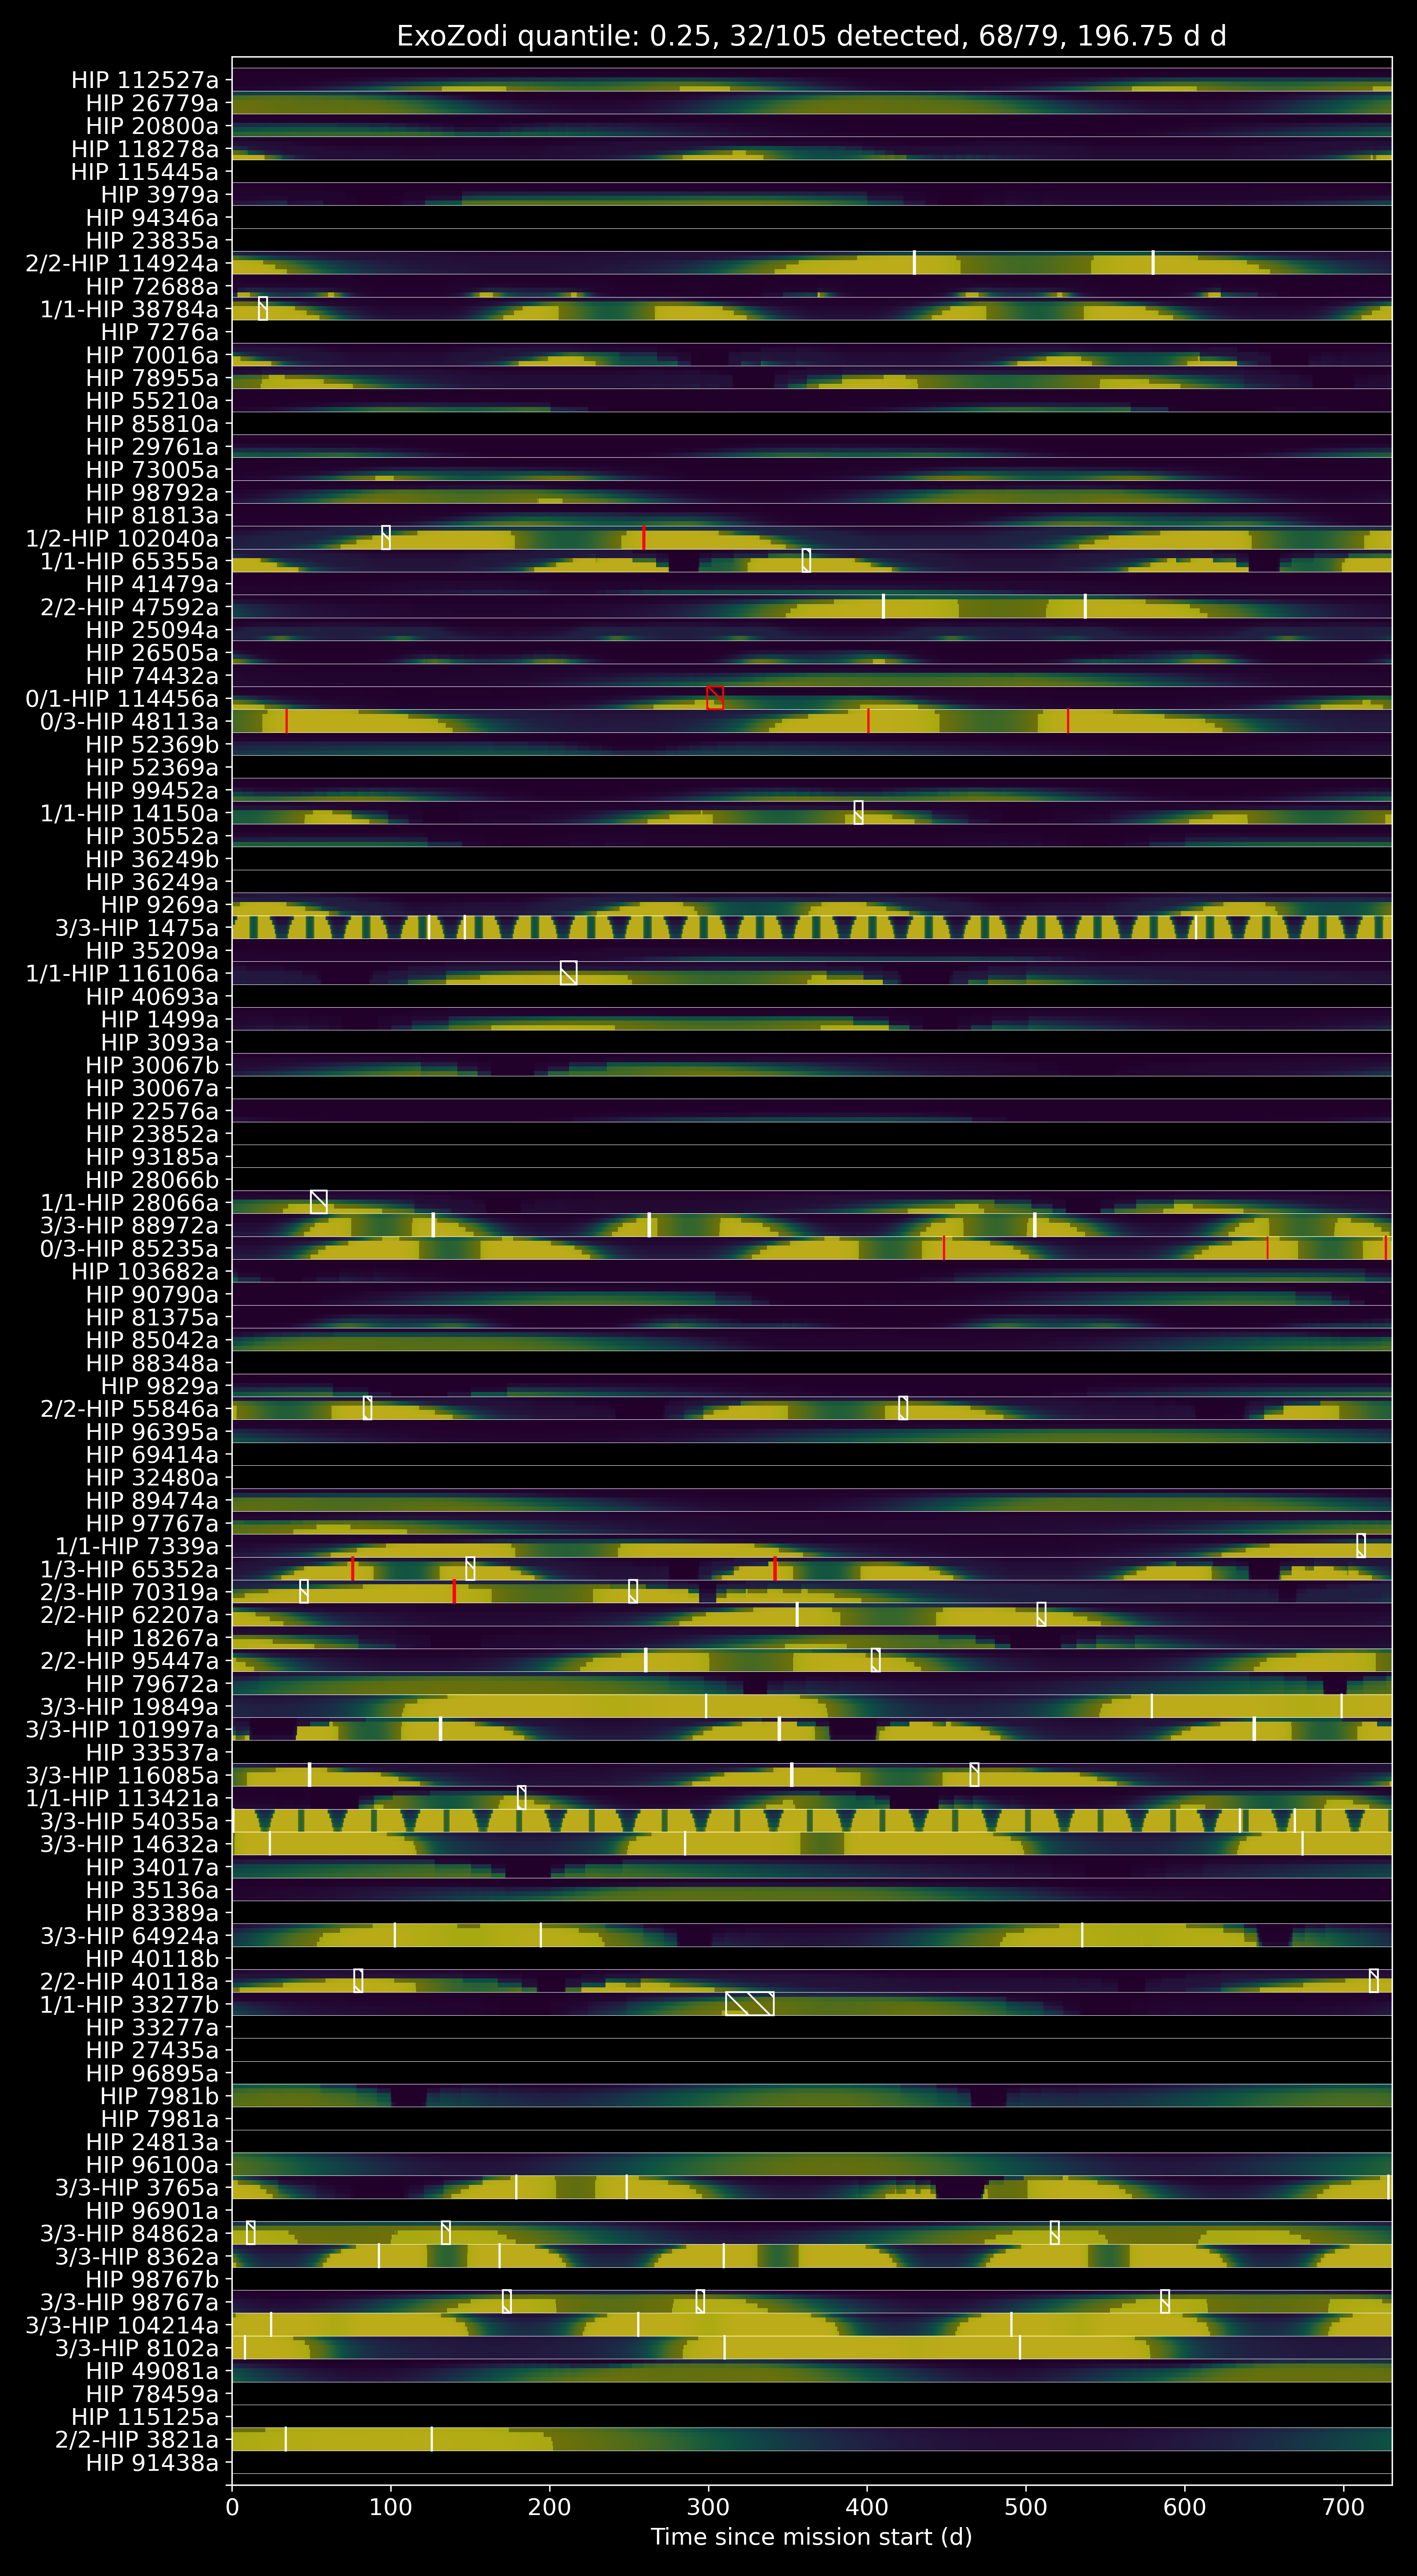
\includegraphics[height=0.9\textheight]{ch4/figures/schedule.png}
  \end{center}
  \caption{
    Schedule created based fits of 3 cm/s EPRV data on 97 stars populated with
    Earth-like planets.
  }
  \label{fig:schedule}
\end{figure}

\begin{figure}
  \begin{center}
    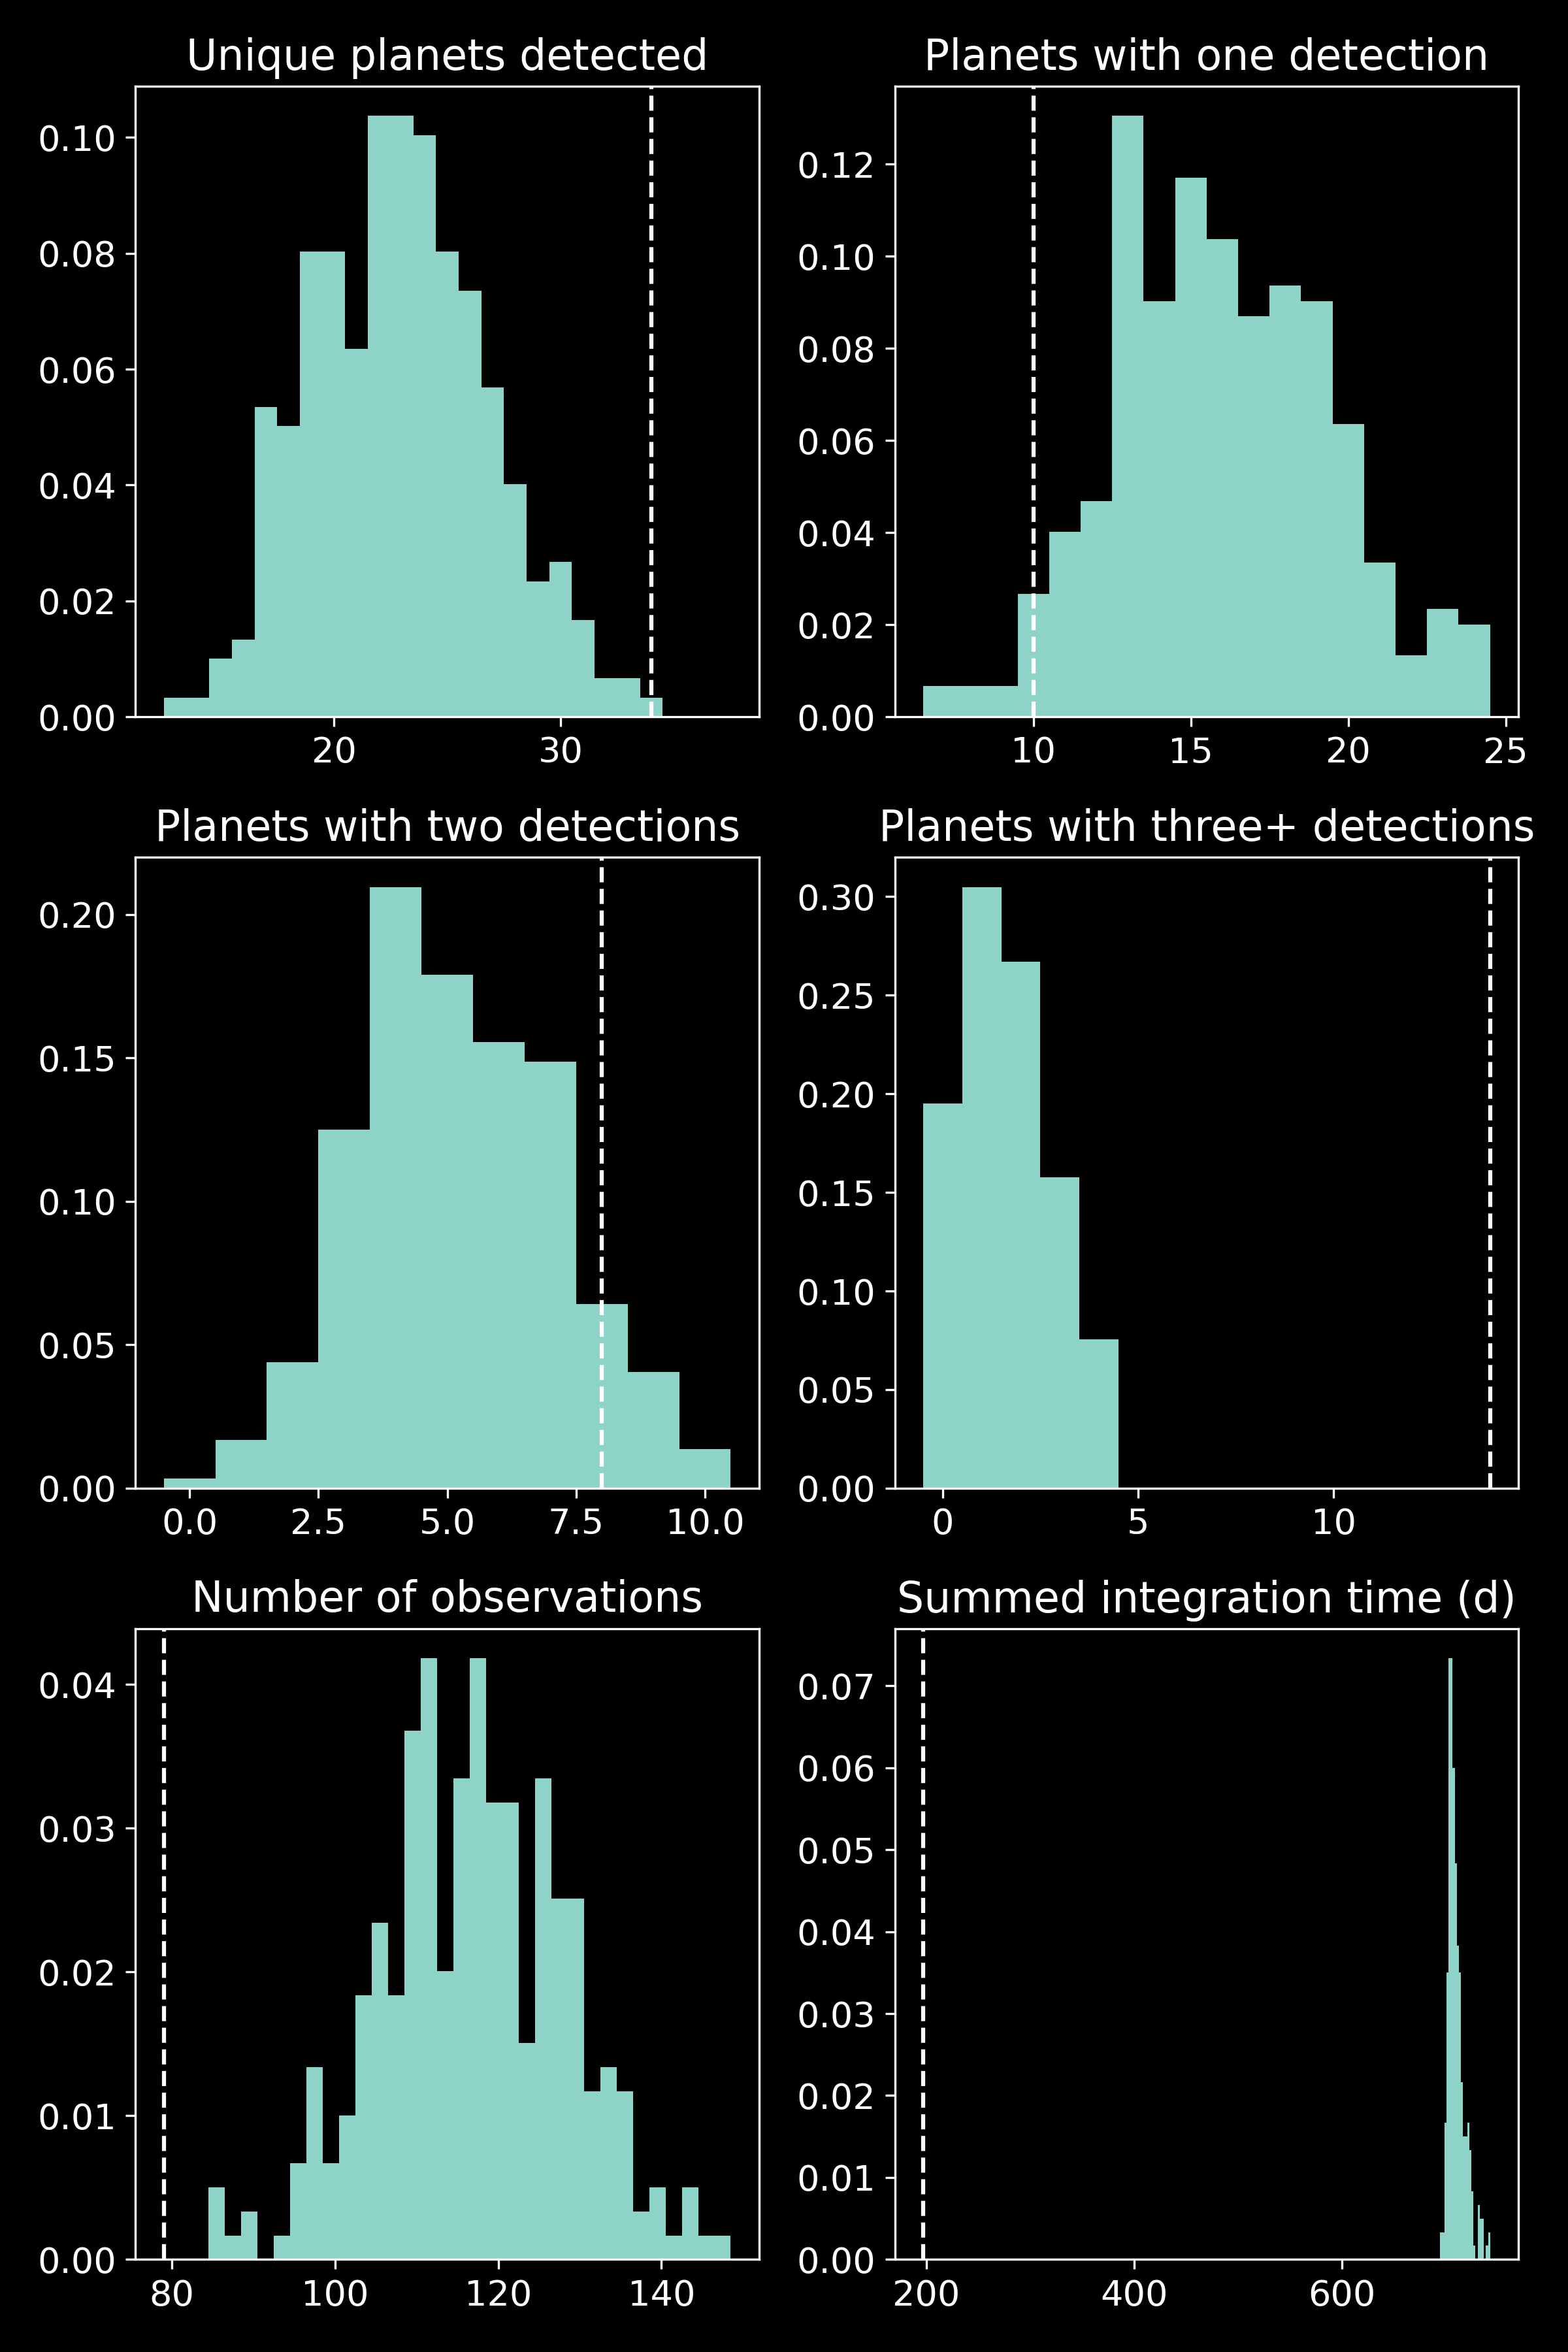
\includegraphics[height=0.75\textheight]{ch4/figures/hist.png}
  \end{center}
  \caption{Comparison between the static observing schedule, dashed line, set by the
  scheduler and a random walk between the 97 stars, histogram. All stars had an Earth-like planet,
  integration times were chosen to reach 25 $\Delta$mag (scaled by the stars luminosity).}
  \label{fig:randomwalkhist}
\end{figure}

An example schedule is shown in \Cref{fig:randomwalkhist}, where 32 of the 105
planets was detected at least once, 79 observations were scheduled, and 68 of
the scheduled observations were successful. In total the scheduler used 196.75
days of integration time out of the allowed two years. It is difficult to find
an analogous comparison in literature to the case we are showing, as previous
studies of RV knowledge fixed the positions of the planets to be the same for
all observations, used a much larger target list, and focused on full
characterization which is not included in this
work\citep{morganExplorationExpectedNumber2022a}. Because of this we compare
our schedule to a random walk scheduler, where we use the same set of planets
and telescope parameters and simulate a mission by choose the next target
randomly for the full mission time. The integration times per target star were
chosen such that instrument could reach $\Delta\textrm{mag}=25$. The results
can be seen in \Cref{fig:randomwalkhist} where our scheduler was able to detect
as many unique planets in 200 days of integration time as the random walk
scheduler detected with 700 days of integration time in its best case scenario.
Additionally the scheduler dramatically out performs a random walk in the
number of planets that it is able to detect three times.

To test the impact of the precision $\sigma$ and the assumed number of zodis in
a planetary system on the scheduler we ran the same situation without redrawing
until an Earth-like planet is in a system. In this way we end up with fewer
total fits, based on the occurrence rate of Earth-like planets,
$\eta_{\oplus}$, which we set to 0.24 in line with
\citep{dulzJointRadialVelocity2020} occurrence rates which was also used in the
EPRV study \citet{morganExplorationExpectedNumber2022a}. We reduce the
computation load as we are interested in the success rate of the fitting
algorithm and the scheduler. We testing the scheduler for 5 $\sigma$ values
(0.1, 0.07, 0.05, 0.03, 0.01 m/s) and 5 $q_\textrm{EZ}$ values (0.05, 0.25,
0.5, 0.75, 0.95) where the $q_\textrm{EZ}$ values map to zodi occurrence rates
used in the \code{EXOSIMS} module \code{Mennesson} based on
\citet{mennessonCONSTRAININGEXOZODIACAL2014} (CHECK with Dmitry that this is where
that fits file comes from). 

The results are shown in \Cref{fig:sigma_nEZ_impact_plots} where the impact of
the $\sigma$ value on the number of Exo-earths fitted is clearly demonstrated.
We see that if a 3 cm/s precision is reached, the value used in the EPRV study
\citet{morganExplorationExpectedNumber2022a}, then we can fit the orbits of
approximately 80 percent of the Earth-like planets. However, if we are limited
to 10 cm/s we will only expect to fit 40 percent of the Earth-like planets. By
then simulating the probability of detection, scheduling, and observation
process calculations we can study how the different $\sigma$ values impact
observation success rate and we see little effect. The $\sigma$
values strongly correlate to the percentage of planets detected, which is unsurprising
given that fewer orbits are fitted.

The assumed number of exozodi has a positive relationship with the observation
success rate and a negative relationship on the mission yield past the 50th
zodi quantile. This shows an interesting trade space where we can better
guarantee the success of an individual observation if we assume high levels of
extra zodiacal light, but this approach ultimately has a negative impact on the
total yield of the mission.

\begin{figure}
  \begin{center}
    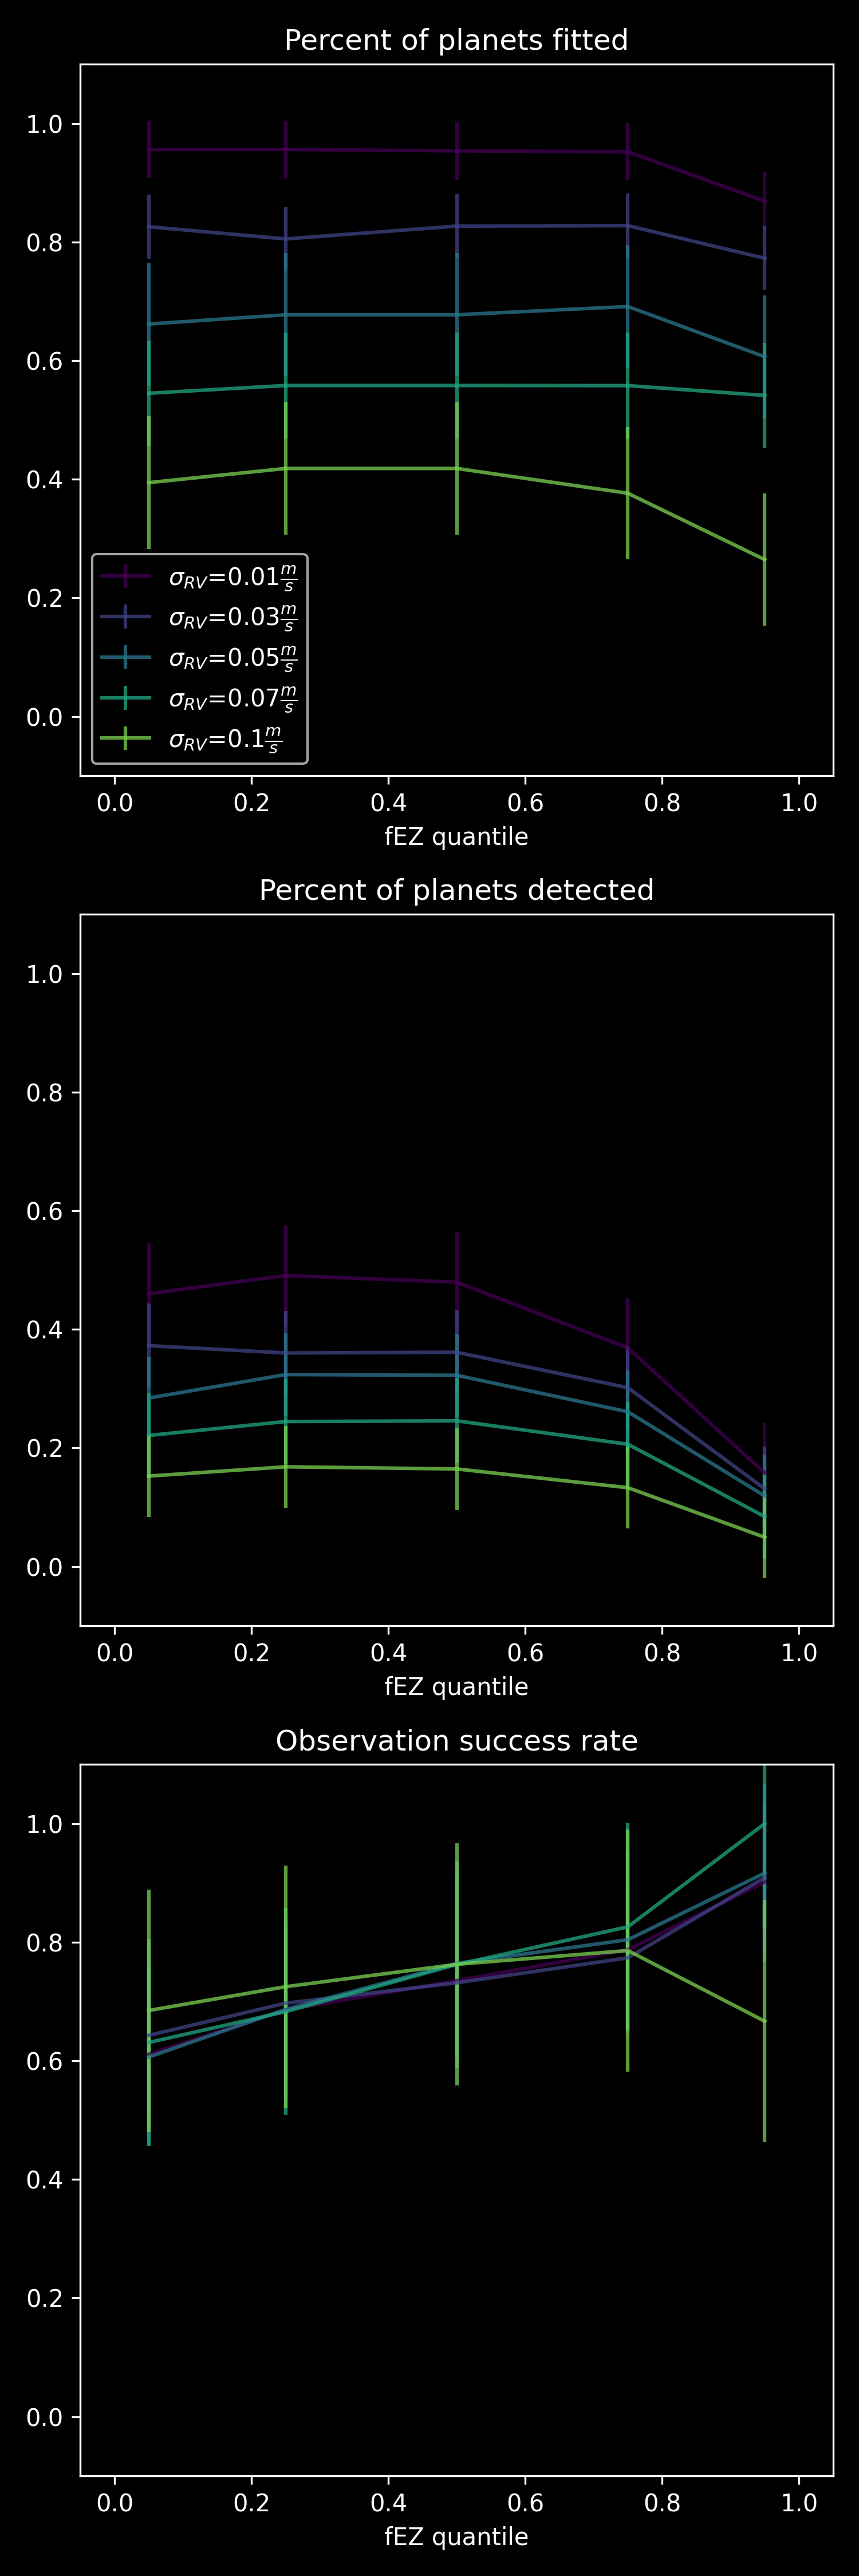
\includegraphics[height=0.9\textheight]{ch4/figures/fEZ_impact.png}
  \end{center}
  \caption{
    Impact of assumption on $\sigma$ and exozodi on scheduler results.
  }
  \label{fig:sigma_nEZ_impact_plots}
\end{figure}

\section{Conclusion}

In this chapter we have demonstrated a method of using constraint programming
to calculate an observing schedule that allows for dynamic variations in the
integration time and observation time for every planet with precursor radial
velocity data. To validate the scheduler we created a tool called \code{RVtoImaging}
that realistically simulates the RV data collection and fitting process,
calculates the probability of detection for a given orbit fit and direct
imaging telescope, schedules observations based on that data, and then uses
mission simulation software to test the scheduled observations. We showed that
our scheduler dramatically out performs a random walk scheduler. This work
proves that we can use the probability of detection metric to schedule direct
imaging observations of exoplanets detected via radial velocity and it shows
how precursor data can be incorporated in direct imaging mission yield
modeling.

More generally, by creating a flexible framework that does full simulations of
the RV observations and fitting process we have created a tool that can answer
many interesting questions in the use of precursor science for a flagship
direct imaging mission such as the Habitable Worlds Observatory. We used a
relatively simple setup in this chapter: a single observing run, no bad
weather, only planets in the habitable zone, and observations were continued
until the direct imaging mission launch. Future work will be on more
complicated scenarios, such as: how many EPRV observations of a planetary
system are required to accurately calculate probability of detection, how does
the planetary occurrence rate model impact which planets are ultimately fitted
via radial velocity, is there there a benefit to prioritizing RV observations
of stars with low completeness because a blind direct imaging search will be
more sensitive to that star.

